%%%%%%%% ICML 2022 EXAMPLE LATEX SUBMISSION FILE %%%%%%%%%%%%%%%%%

\documentclass[nohyperref]{article}

% Recommended, but optional, packages for figures and better typesetting:
\usepackage{microtype}
\usepackage{graphicx}
\usepackage{subfigure}
\usepackage{booktabs} % for professional tables

% hyperref makes hyperlinks in the resulting PDF.
% If your build breaks (sometimes temporarily if a hyperlink spans a page)
% please comment out the following usepackage line and replace
% \usepackage{icml2022} with \usepackage[nohyperref]{icml2022} above.
\usepackage{hyperref}


% Attempt to make hyperref and algorithmic work together better:
\newcommand{\theHalgorithm}{\arabic{algorithm}}

% Use the following line for the initial blind version submitted for review:
%\usepackage{icml2022}

% If accepted, instead use the following line for the camera-ready submission:
\usepackage[accepted]{icml2022}

% For theorems and such
\usepackage{amsmath}
\usepackage{amssymb}
\usepackage{mathtools}
\usepackage{amsthm}

% if you use cleveref..
\usepackage[capitalize,noabbrev]{cleveref}

%%%%%%%%%%%%%%%%%%%%%%%%%%%%%%%%
% THEOREMS
%%%%%%%%%%%%%%%%%%%%%%%%%%%%%%%%
\theoremstyle{plain}
\newtheorem{theorem}{Theorem}[section]
\newtheorem{proposition}[theorem]{Proposition}
\newtheorem{lemma}[theorem]{Lemma}
\newtheorem{corollary}[theorem]{Corollary}
\theoremstyle{definition}
\newtheorem{definition}[theorem]{Definition}
\newtheorem{assumption}[theorem]{Assumption}
\theoremstyle{remark}
\newtheorem{remark}[theorem]{Remark}

% Todonotes is useful during development; simply uncomment the next line
%    and comment out the line below the next line to turn off comments
%\usepackage[disable,textsize=tiny]{todonotes}
\usepackage[textsize=tiny]{todonotes}


% The \icmltitle you define below is probably too long as a header.
% Therefore, a short form for the running title is supplied here:
\icmltitlerunning{Extremum Seeking Gradient}

\begin{document}

\twocolumn[
\icmltitle{Extremum Seeking Gradient \\ Machine Learning without Backpropagation}

% It is OKAY to include author information, even for blind
% submissions: the style file will automatically remove it for you
% unless you've provided the [accepted] option to the icml2022
% package.

% List of affiliations: The first argument should be a (short)
% identifier you will use later to specify author affiliations
% Academic affiliations should list Department, University, City, Region, Country
% Industry affiliations should list Company, City, Region, Country

% You can specify symbols, otherwise they are numbered in order.
% Ideally, you should not use this facility. Affiliations will be numbered
% in order of appearance and this is the preferred way.
\icmlsetsymbol{equal}{*}

\begin{icmlauthorlist}
\icmlauthor{Or Dicker}{yyy}
\icmlauthor{David Prichen}{yyy}
%\icmlauthor{Firstname3 Lastname3}{comp}
%\icmlauthor{Firstname4 Lastname4}{sch}
%\icmlauthor{Firstname5 Lastname5}{yyy}
%\icmlauthor{Firstname6 Lastname6}{sch,yyy,comp}
%\icmlauthor{Firstname7 Lastname7}{comp}
%\icmlauthor{}{sch}
%\icmlauthor{Firstname8 Lastname8}{sch}
%\icmlauthor{Firstname8 Lastname8}{yyy,comp}
%\icmlauthor{}{sch}
%\icmlauthor{}{sch}
\end{icmlauthorlist}

\icmlaffiliation{yyy}{Department of Electrical Engineering, Tel Aviv University}
%\icmlaffiliation{comp}{Company Name, Location, Country}
%\icmlaffiliation{sch}{School of ZZZ, Institute of WWW, Location, Country}

\icmlcorrespondingauthor{Or Dicker}{or.dicker@gmail.co.il}
\icmlcorrespondingauthor{David Prichen}{first2.last2@gmail.co.il}

% You may provide any keywords that you
% find helpful for describing your paper; these are used to populate
% the "keywords" metadata in the PDF but will not be shown in the document
\icmlkeywords{Machine Learning, ICML, Extremum Seeking}

\vskip 0.3in
]

% this must go after the closing bracket ] following \twocolumn[ ...

% This command actually creates the footnote in the first column
% listing the affiliations and the copyright notice.
% The command takes one argument, which is text to display at the start of the footnote.
% The \icmlEqualContribution command is standard text for equal contribution.
% Remove it (just {}) if you do not need this facility.

\printAffiliationsAndNotice{}  % leave blank if no need to mention equal contribution
%\printAffiliationsAndNotice{\icmlEqualContribution} % otherwise use the standard text.

\begin{abstract}

  \begin{figure}[ht]
\vskip 0.2in
\begin{center}
\centerline{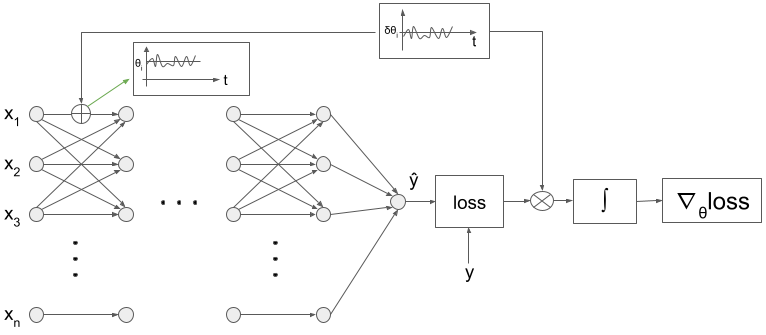
\includegraphics[width=\columnwidth]{images/ESG-scheme.png}}
\caption{}
   \label{ESG-sheme}
\end{center}
\vskip -0.2in
\end{figure}
\end{abstract}

\section{Introduction}
\subsection{Analog Neural Network}
Analog neural networks represent a fascinating and promising paradigm within the realm of artificial neural networks. In contrast to their digital counterparts, which operate with discrete values, analog neural networks leverage continuous, analog signals in both the input and computation stages, emulating the behavior of biological neurons more closely. This unique approach allows analog neural networks to potentially overcome certain limitations of digital systems, such as precision constraints and energy efficiency. Furthermore, analog networks can harness the principles of neuromorphic computing, mimicking the brain's computational processes and offering potential advantages in tasks involving real-time sensory perception and complex, low-power computations. Despite facing challenges related to noise and signal fidelity, analog neural networks have garnered significant attention for their potential to revolutionize fields like edge computing, sensor fusion, and neuromorphic hardware design. As researchers continue to explore and refine the capabilities of analog neural networks, they hold the promise of ushering in a new era of efficient, brain-inspired computing systems with applications spanning from machine learning to cognitive science and beyond.
While analog neural networks offer intriguing prospects, they are not without significant challenges during the learning phase. One of the primary downsides in this context is the limited flexibility and adaptability of analog systems compared to their digital counterparts. Analog networks often struggle to implement complex learning algorithms, particularly those involving backpropagation, which heavily rely on precise weight updates and gradient computations. The continuous nature of analog signals can introduce difficulties in controlling and fine-tuning synaptic strengths, which are essential for effective learning. Moreover, analog networks are susceptible to noise, parameter drift, and variations in device characteristics, making it challenging to maintain stable and consistent learning processes over time. These limitations pose significant hurdles when aiming to train analog neural networks for complex tasks, potentially hindering their broader adoption in applications requiring sophisticated learning capabilities. Researchers are actively addressing these challenges to unlock the full potential of analog neural networks while mitigating their downsides during the learning phase.

The paper by IBM \cite{le202364} represents a significant advancement in the field of hardware acceleration for artificial intelligence (AI) and deep learning. The core focus of this research centers on the development of a novel compute chip architecture that combines mixed-signal processing techniques with emerging phase-change memory technology to enhance the efficiency of deep neural network inference tasks.
The integration of phase-change memory into the chip architecture is particularly noteworthy. Phase-change memory is an emerging non-volatile memory technology with the potential to revolutionize AI hardware due to its low power consumption, high density, and fast access times. This paper demonstrates the practical feasibility of leveraging phase-change memory as a key component in an in-memory computing system tailored for deep neural network inference.
The use of mixed-signal processing further extends the capabilities of this chip. By combining analog and digital processing elements, the 64-core architecture achieves a balance between computational power and energy efficiency, a crucial consideration for edge and embedded AI applications. This mixed-signal approach allows for efficient processing of neural network workloads, enabling real-time inference in power-constrained environments.
Overall, the paper represents a notable step forward in the pursuit of hardware solutions that can accelerate deep learning tasks while remaining energy-efficient. It highlights the potential of phase-change memory and mixed-signal processing techniques in shaping the future of AI hardware, with implications for a wide range of applications, including autonomous vehicles, IoT devices, and edge computing platforms. The research presented in this paper serves as a valuable contribution to the ongoing efforts to make deep learning more accessible and efficient for a variety of real-world scenarios.

\subsubsection{Photonic Neural Network}
Photonic neural networks (PNNs) constitute a transformative paradigm in the domain of artificial neural networks, leveraging the principles of photonics for computational and information processing tasks. Unlike their electronic counterparts, which employ electrons for information transmission, PNNs utilize photons, the fundamental particles of light, to perform a wide array of complex operations. This departure from traditional electronic computing offers several distinct advantages, notably in terms of speed and energy efficiency.
One of the key advantages of photonic neural networks lies in their inherent parallelism. Photons can traverse multiple paths simultaneously, allowing for massively parallel computations that excel in tasks involving large-scale data processing, such as image recognition and natural language understanding. This parallelism can significantly reduce computational time, making PNNs particularly well-suited for applications where real-time processing is critical.
Moreover, photonic systems are known for their ultra-fast data transmission speeds. The propagation of light through optical waveguides occurs at a velocity close to the speed of light, enabling rapid information exchange between network components. This high-speed operation is advantageous in scenarios requiring low-latency responses, such as autonomous vehicles and telecommunications.
Furthermore, PNNs demonstrate inherent resistance to electromagnetic interference and reduced heat generation compared to their electronic counterparts. This resilience to interference makes them ideal for applications where reliability and stability are paramount, such as in aerospace and defense systems.
The experimental realization of in situ backpropagation for deep learning in photonic neural networks \cite{Pai_2023} signifies a groundbreaking achievement at the intersection of photonics and artificial intelligence. This pioneering research demonstrates the feasibility of employing photonic components to execute the essential backpropagation algorithm within the neural network itself, a task traditionally handled in electronic domains. By harnessing the unique properties of light, this approach offers the potential for ultra-high-speed and energy-efficient training of deep neural networks. This breakthrough not only addresses key challenges in the convergence of photonic and electronic components but also paves the way for the development of photonic neural networks with real-time learning capabilities. As the field of optical computing continues to evolve, the experimental realization of in situ backpropagation holds immense promise for advancing the capabilities of deep learning and expanding the horizons of photonic neural networks in various applications, from data processing to cognitive computing and beyond.
\subsection{What is wrong with backpropagation}
Hinton claims that propagation can't be how the brain learns as a model e despite considerable effort to
invent ways in which it could be implemented by real neurons. There is no convincing evidence
that cortex explicitly propagates error derivatives or stores neural activities for use in a subsequent
backward pass. The top-down connections from one cortical area to an area that is earlier in the
visual pathway do not mirror the bottom-up connections as would be expected if backpropagation
was being used in the visual system. Instead, they form loops in which neural activity goes through
about half a dozen cortical layers in the two areas before arriving back where it started.
Backpropagation through time as a way of learning sequences is especially implausible. To deal with
the stream of sensory input without taking frequent time-outs, the brain needs to pipeline sensory
data through different stages of sensory processing and it needs a learning procedure that can learn
on the fly. The representations in later stages of the pipeline may provide top-down information
that influences the representations in earlier stages of the pipeline at a later time step, but the
perceptual system needs to perform inference and learning in real time without stopping to perform
backpropagation.A further serious limitation of backpropagation is that it requires perfect knowledge of the computation
performed in the forward pass in order to compute the correct derivatives If we insert a black
box into the forward pass, it is no longer possible to perform backpropagation unless we learn a
differentiable model of the black box.
We believe that ESG learning algorithm \cref{alg:ESG-analog} could overcame these limitation and, but different hardware is needed to compete with backpropagation performance.   

\subsection{Extremum Seeking Control}
Extremum seeking control is a dynamic optimization technique employed in control systems to seek and maintain the optimal operating point of a system, often in the presence of changing or uncertain conditions. It operates by systematically perturbing a control input and observing the resulting system response to detect changes in a chosen performance metric. By continuously adjusting the control input in the direction that improves or maximizes the observed metric, extremum seeking control can adapt to variations in the system and ensure optimal performance. This approach is particularly valuable in applications where precise modeling of system dynamics is challenging, offering a versatile and robust solution for optimizing processes and systems in real-time.

\begin{figure}[ht]
\vskip 0.2in
\begin{center}
\centerline{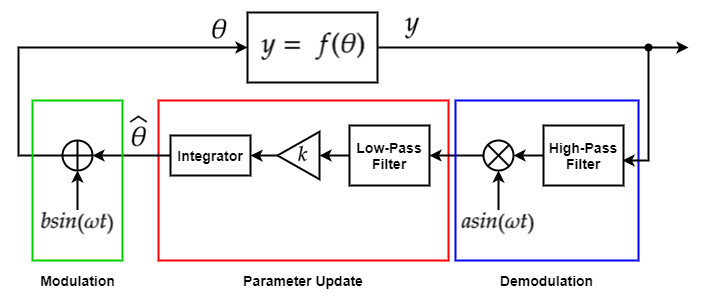
\includegraphics[width=\columnwidth]{images/esc_static_optimization.png}}
\caption{}
\end{center}
\vskip -0.2in
\end{figure}

\begin{figure}[ht]
\vskip 0.2in
\begin{center}
\centerline{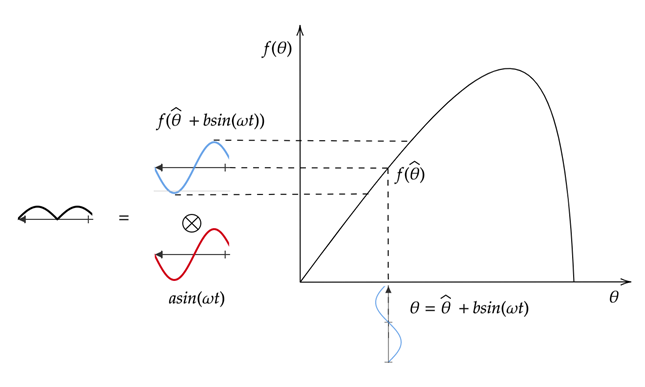
\includegraphics[width=\columnwidth]{images/esc_increasing_objective.png}}
\caption{}
\end{center}
\vskip -0.2in
\end{figure}


\section{Algorithm}
\begin{figure*}[ht]
\vskip 0.2in
\begin{center}
\centerline{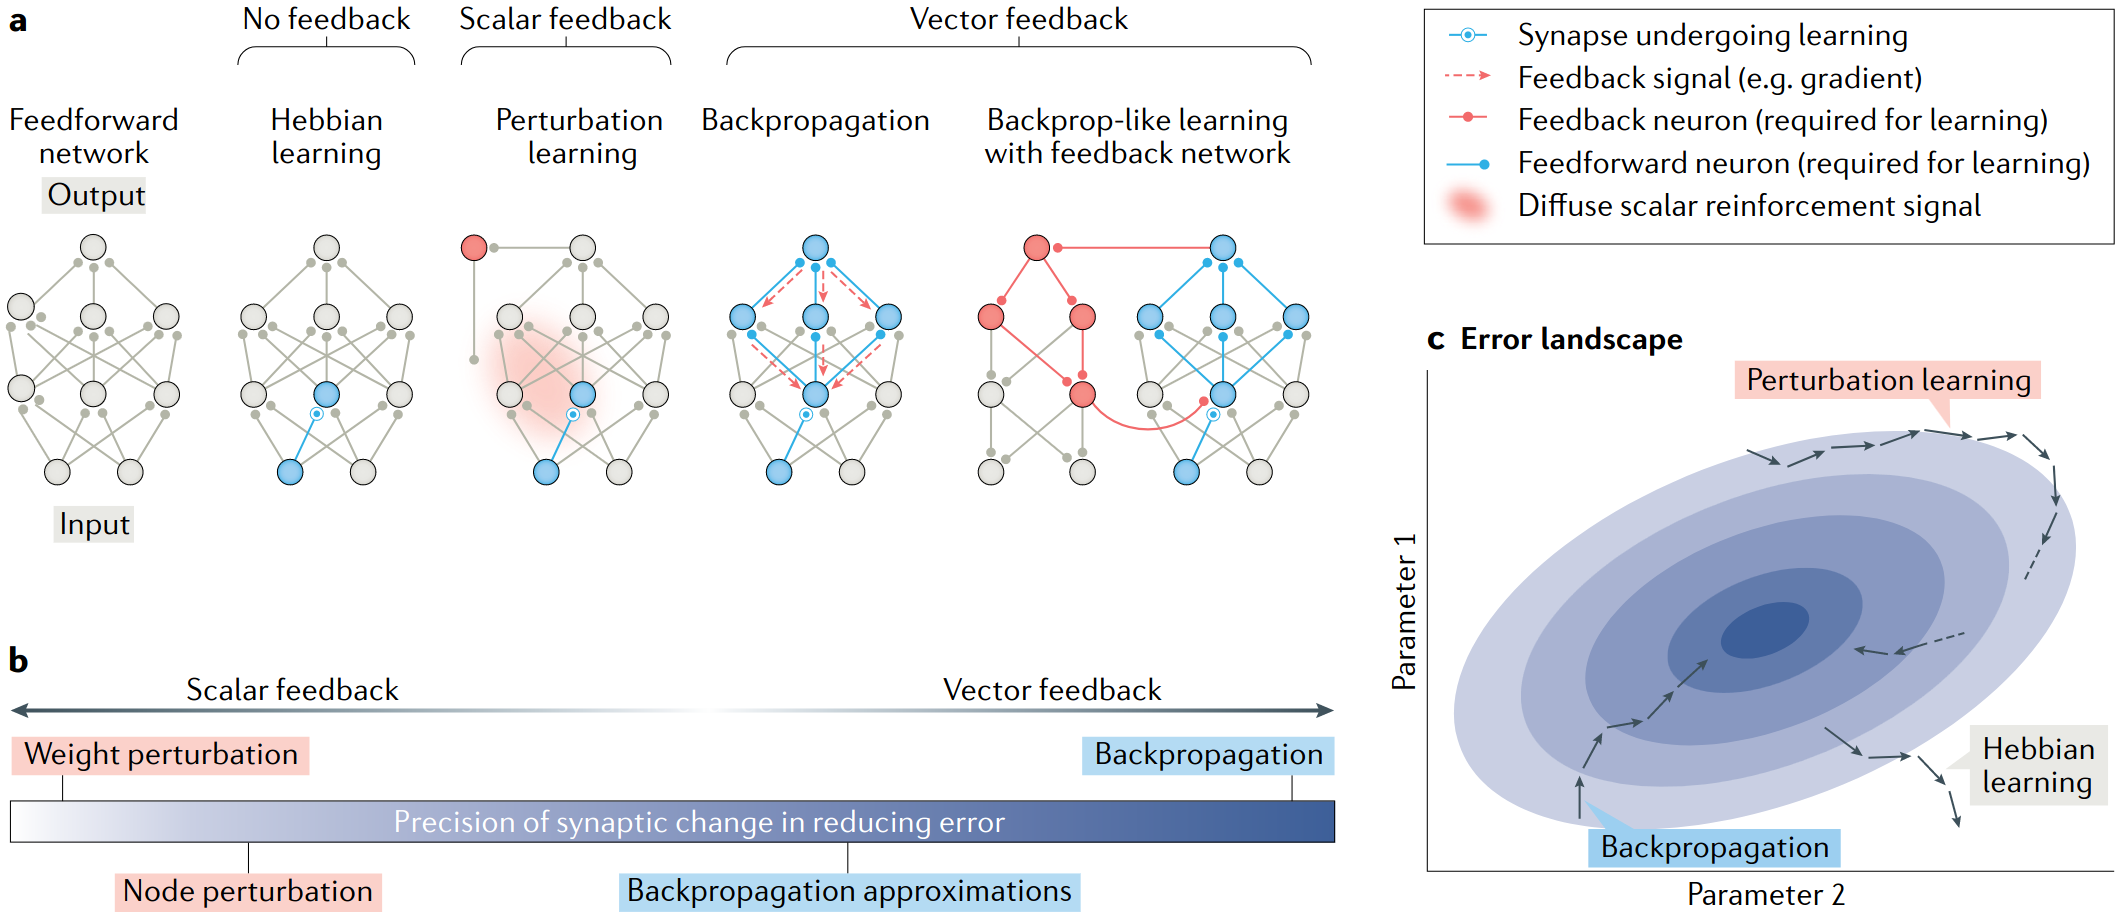
\includegraphics[width=2\columnwidth]{images/grad_landscape.png}}
\caption{\textbf{A spectrum of learning algorithms \cite{journe2022hebbian}} | From left to right, a neural network processes data through simple computational units and adjusts the connections (synapses) between these units to enhance its performance on a given task. Traditional Hebbian learning, which strengthens synapses when a presynaptic neuron consistently contributes to a postsynaptic neuron's firing, cannot effectively modify certain synapses because it doesn't account for their downstream impact on the network's overall output.}
\label{grad_landscape}
\end{center}
\vskip -0.2in
\end{figure*}

\subsection{Backpropagation}
Backpropagation\cref{alg:BP}, a fundamental algorithm in the field of deep learning, offers substantial advantages in terms of computational efficiency, especially when dealing with inputs of significantly larger dimensions than the network's initial layer. This characteristic becomes particularly relevant in today's era of big data and complex information processing tasks.

One of the primary advantages of backpropagation in such scenarios is its ability to efficiently calculate gradients for each layer of a deep neural network. When the input dimensionality is high, traditional optimization techniques become computationally prohibitive due to the curse of dimensionality. However, backpropagation mitigates this challenge by propagating errors backward through the layers, effectively distributing the computation of gradients across the network. This distributed computation not only reduces the computational burden but also allows for parallelization, which can be leveraged with modern hardware, such as GPUs and TPUs, to expedite the training process.

\begin{algorithm}[tb]
     \caption{Backpropagation}
   \label{alg:BP}

  \begin{algorithmic}
\STATE Compute the error at the output layer:
\STATE $\delta^{(L)} = \nabla_a \mathcal{L} \odot \sigma'(z^{(L)})$
\FOR{each layer $l$ from $L-1$ to $1$}
    \STATE Backpropagate the error through the layers:
    \STATE $\delta^{(l)} = ((W^{(l+1})^T \delta^{(l+1)}) \odot \sigma'(z^{(l)})$
    \STATE Calculate the gradients of the weights and biases:
    \STATE $\nabla W^{(l)} = \delta^{(l)}(a^{(l-1)})^T$
    \STATE $\nabla b^{(l)} = \delta^{(l)}$
\ENDFOR    
\end{algorithmic}
\end{algorithm}



\subsection{Forward Forward Algorithm(Hebbian Learning)}
Hebbian learning\cite{journe2022hebbian} is a fundamental concept in neuroscience and artificial neural networks, describing a synaptic plasticity rule that governs how the strength of connections between neurons evolves over time. Named after the psychologist Donald Hebb, it is often summarized by the phrase "cells that fire together, wire together." In essence, if two neurons are frequently active at the same time, the synaptic connection between them is strengthened. This process reinforces the association between neurons and is believed to play a critical role in learning and memory formation. Hebbian learning has also influenced the development of artificial neural networks, where it has been used as a foundational principle for training models to capture patterns and relationships in data.

The Forward-Forward algorithm \cite{hinton2022forward}, introduced by Geoffrey Hinton, represents a novel and innovative approach to deep learning that draws inspiration from Boltzmann machines and Noise Contrastive Estimation. Unlike traditional backpropagation, this method employs two forward passes that operate symmetrically but on distinct datasets with opposing objectives. The positive pass refines network weights to enhance representations for real data, while the negative pass adjusts weights to diminish quality for negative data. This unique framework allows for the exploration of various quality metrics. The ultimate aim of the Forward-Forward algorithm is to effectively classify input vectors as positive or negative data based on a logistic function applied to the quality metric, making it a promising and versatile addition to the arsenal of deep learning techniques.

Let us suppose that the goodness function for a layer is simply the sum of the squares of the activities
of the rectified linear neurons in that layer4 The aim of the learning is to make the goodness be
well above some threshold value for real data and well below that value for negative data. More
specifically, the aim is to correctly classify input vectors as positive data or negative data when the probability that an input vector is positive (i. e. real) is given by applying the logistic function, $\sigma$ to the goodness, minus some threshold $\theta$
$$p(positive) = \sigma(\sum_{j}y^{2}_{j}-\theta)$$
where $y_{j}$ is the activity of hidden unit $j$ before layer normalization. 

\begin{figure}[ht]
\vskip 0.2in
\begin{center}
\centerline{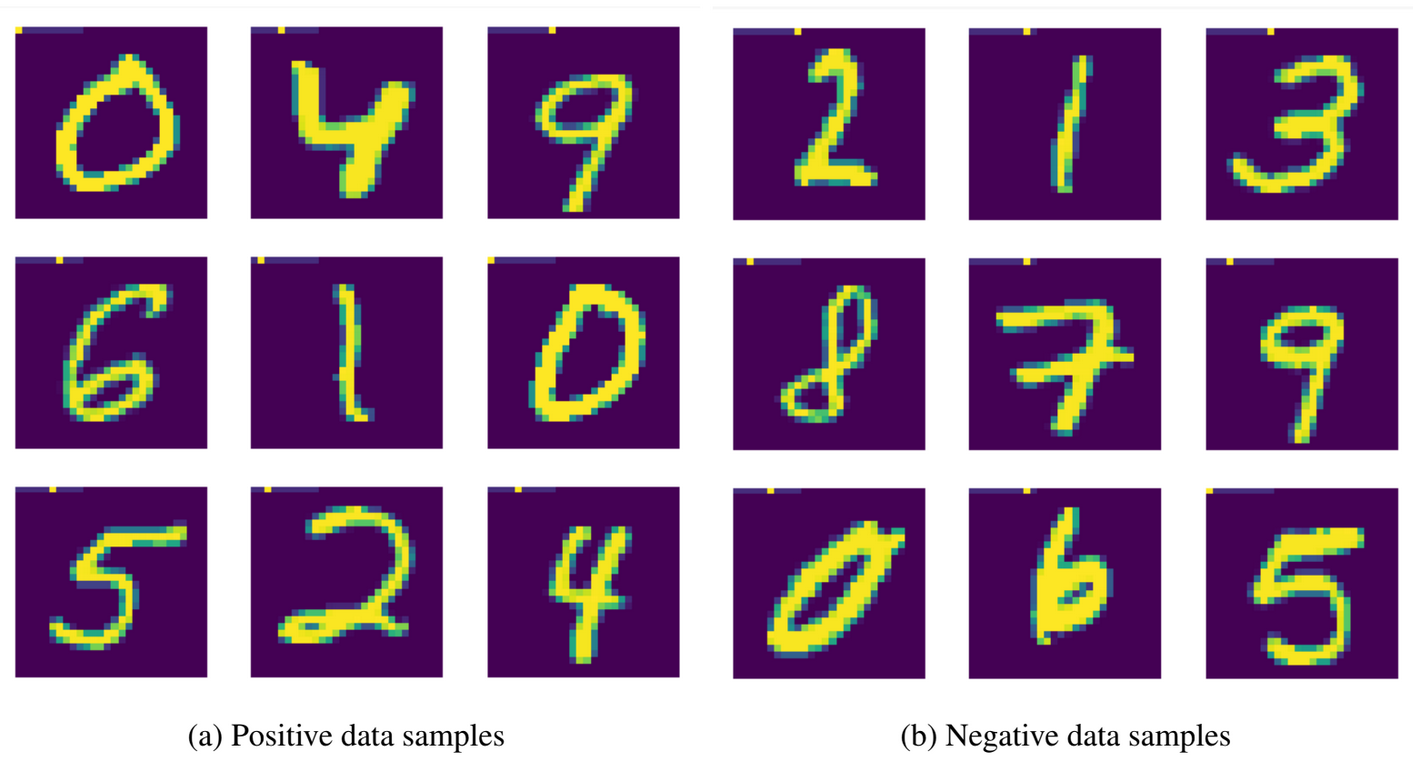
\includegraphics[width=\columnwidth]{images/FF_embedding.png}}
\caption{Data embedding for Forward Forward algorithm. The label can be seen in the top left 10 pixels}
  \label{fig:FF_embed}
\end{center}
\vskip -0.2in
\end{figure}


\begin{algorithm}[tb]
   \caption{Forward Forward}
   \label{alg:FF}
\begin{algorithmic}
   \STATE {\bfseries Input:} dataset $\{x_{i},y_{i}\}$, NN architecture $f(x;\theta)$, NN parameters $\theta$, goodness $\theta(\hat{y},y)$ 
   \FOR{each training example $(x^{(i)}, y^{(i)})$}
   \STATE \textbf{Positive Pass:}
   \STATE embed $(x^{(i)}, y^{(i)})$ together like fig \ref{fig:FF_embed}
    \STATE Perform a forward pass with real data to compute the goodness metric.
    \STATE Adjust the weights to increase the goodness above a threshold for real data.
    \STATE \textbf{Negative Pass:}
    \STATE embed $(x^{(i)}, \tilde{y}^{(i)})$  where $\tilde{y}$ is random
    \STATE Perform a forward pass with "negative data" to compute the goodness metric.
    \STATE Adjust the weights to decrease the goodness below the threshold for negative data.
\ENDFOR
\end{algorithmic}
\end{algorithm}

\subsection{Simultaneous-Perturbation Stochastic
Approximation (SPSA) (gradient part)}
Simultaneous Perturbation Stochastic Approximation (SPSA)\cref{alg:SPSA} is a powerful optimization technique used primarily in scenarios where obtaining precise gradient information for a complex objective function is challenging or computationally expensive. SPSA is particularly valuable in the field of optimization and has found applications in various domains, including engineering, machine learning, and operations research.

At its core, SPSA is a gradient-free optimization method designed to efficiently search for the optimal solution within a parameter space, typically characterized by a high dimensionality. This technique is particularly well-suited for scenarios where the underlying objective function is non-convex, noisy, or lacks a readily available closed-form expression.

The distinguishing feature of SPSA is its use of simultaneous perturbations, where it estimates the gradient of the objective function by evaluating the function at two different points, perturbed in opposite directions along each parameter axis. By analyzing the difference in function values resulting from these perturbations, SPSA approximates the gradient direction, allowing it to iteratively update the parameter values towards the optimum.

\begin{algorithm}[tb]
   \caption{SPSA}
   \label{alg:SPSA}
\begin{algorithmic}
  \STATE {\bfseries Input:} dataset $\{x_{i},y_{i}\}$, NN architecture $f(x;\theta)$, NN parameters $\theta$, Loss function $L(\hat{y},y)$, sigma $\sigma$, $N$
  \STATE {\bfseries Output:} $grad$
  \STATE update $\delta \theta$
  \STATE $L_{+} \leftarrow L(y,f(x;\theta+\delta \theta))$
  \STATE $L_{-} \leftarrow L(y,f(x;\theta-\delta \theta))$
  \STATE $grad_{i} = \frac{L_{+}-L_{-}}{\delta\theta_{i}}$
  \STATE return $grad$

\end{algorithmic}
\end{algorithm}


\subsection{Extremum Seeking Gradient}
We commence with the fundamental premise that we possess hardware equipped with programmable parameters, such as weights and biases, enabling it to execute inference tasks. Our objective is to extend this hardware's capabilities with minimal modifications so that it can undergo training via gradient descent. We will illustrate how to set up the hardware in a manner that facilitates the network's collective execution of gradient descent without relying on backpropagation.
As an example, assume we have a hardware instantiation of a feedforward multi-layer neural network as shown in figure \ref{ESG-sheme}. The hardware takes time-varying inputs ${x_{n}(t)}$ and ground truth $y(t)$ and as parameters $\theta$ the network output $\hat{y}$ and a $loss(\hat{y}, y)$ objective function.
We introduce noise $\delta\theta$ to the parameters $\theta$, where $E[\delta\theta]=0$ and $E[\delta\theta^{2}]=I\sigma$. Therefore, the output of the network is $\hat{y} = NN(x;\theta+\delta\theta)$. Following the scheme we calculate $loss(\hat{y},y)\cdot \delta\theta$ and taking the average. On the next section we will prove why this value convergence to the $\nabla loss_{\theta}$.
ESG\cref{alg:ESG-analog} allows us to calculate the gradient of any neural network without inverting the computational graph and using single value to propagate backwards (instead of many values like in backpropagation).
This flexible method allow us to traing Analog neural network and photonic neural network quite naturally.
\begin{algorithm}[tb]
   \caption{Extermum Seeking Gradient-Analog}
   \label{alg:ESG-analog}
\begin{algorithmic}
  \STATE {\bfseries Input:} dataset $\{x_{i},y_{i}\}$, NN architecture $f(x;\theta)$, NN parameters $\theta$, Loss function $L(\hat{y},y)$, sigma $\sigma$, $T$, high pass filter $HPF$
  \STATE {\bfseries Output:} $grad$ 
   \STATE $L_{0} = L(y,f(x;\theta))$
   \STATE initialize $grad \leftarrow 0$
   \FOR{$i=1$ {\bfseries to} $T$}
   \STATE update $\delta\theta$
   \STATE $e \leftarrow L(y,f(x;\theta+\delta \theta))\cdot\delta \theta*HPF$
   \STATE $grad \leftarrow \int_{0}^{T}e dt $ 
   \ENDFOR
   \STATE return $grad/T/\sigma^{2}$
\end{algorithmic}
\end{algorithm}


In order to check our method, we developed a digital version of the algorithm\cref{alg:ESG-digital}. The main difference is that the digital version can work on GPU and enable us to test the method on classical machine learning dataset like CIFAR.
The algorithm impemented using JuliaLang\cite{Julia-2017} and Lux.jl\cite{pal2023lux} which allowed us to run both on the CPU and GPU seamlessly and making direct manipulation on the network parameters $\theta$.
\begin{algorithm}[tb]
   \caption{Extermum Seeking Gradient-Digital}
   \label{alg:ESG-digital}
\begin{algorithmic}
  \STATE {\bfseries Input:} dataset $\{x_{i},y_{i}\}$, NN architecture $f(x;\theta)$, NN parameters $\theta$, Loss function $L(\hat{y},y)$, sigma $\sigma$, $N$
  \STATE {\bfseries Output:} $grad$  
   \STATE $L_{0} = L(y,f(x;\theta))$
   \STATE initialize $grad \leftarrow 0$
   \FOR{$i=1$ {\bfseries to} $N$}
   \STATE update $\delta\theta$
   \STATE $grad \leftarrow grad + (L(y,f(x;\theta+\delta \theta))-L_{0})\cdot\delta \theta$
   \ENDFOR
   \STATE return $grad/N/\sigma^{2}$
\end{algorithmic}
\end{algorithm}


\subsubsection{Gradient convergence}
First, we will show that ESG is converging to the true gradient.
Let's assume that $\hat{y} = NN(x;\theta)$ where $NN$ is feed-forward neural network, $\hat{y}$ is the output, $x$ is input, and $\theta$ is the network parameters.
We desire to calculate the gradient of the loss function $loss(NN(x_{i};\theta),y_{i})$ where ${x_{i},y_{i}}$ is a pair of input ($x$) and ground truth output($y$).
let's define $f(\theta) \coloneqq loss(NN(x_{i};\theta),y_{i})$ for fixed ${x_{i},y_{i}}$.
We will notice that $\theta \in \mathbb{R}^{n} $ where $n$ is the network parameters, $f \in \mathbb{R}^{n}\rightarrow\mathbb{R}$.
Let's define $\delta\theta \in \mathbb{R}^{n}$ a vector of $n$ random variables with $E[\delta\theta]=0$ and $E[\delta\theta \cdot \delta\theta^{T}]=I\sigma^{2}$.
Let's evaluate:
$$E[f(\theta+\delta\theta)\delta\theta]$$
using Taylor Series, now we will use expectation linearity and neglect the $O(\delta\theta^{2})$ term.
$$=E[(f(\theta)+\delta\theta^{T} \nabla f(\theta)+O(\delta\theta^{2}))\cdot \delta\theta)]$$
$$=E[f(\theta)\cdot \delta\theta]+E[\delta\theta^{T} \nabla f(\theta)\cdot \delta\theta]$$
Let's remember that $\delta\theta^{T} \nabla f(\theta) \in \mathbb{R}$ and $f(\theta)$ is deterministic.
$$=f(\theta)E[\delta\theta]+E[\delta\theta \cdot \delta\theta^{T}] \nabla f(\theta)$$
Using the properties of $\delta\theta$ we get
$$E[f(\theta+\delta\theta)\delta\theta]= \sigma^{2}\nabla f(\theta)$$
Now let's replace the expectation with the arithmetic mean
$$\nabla f(\theta) \approx \frac{1}{N\sigma^{2}}\sum^{N}_{n=1} f(\theta+\delta\theta)\cdot \delta\theta$$



\section{Experiments}
\subsection{Polynomial Fit}
\subsection{Non Differential activation function}
\subsection{Spiral (LSTM)}
\subsection{MNIST}
\subsection{CIFAR}


\section{Memory Efficient Learning}
While trying to improve the memory usage of ESG (the digital version) we tough about a zero order algorithm.
While trying to implement it we stumped upon MeZO \cite{malladi2023finetuning} which does exactly what we meant to do.  
\subsection{MeZO}
Fine-tuning language models (LMs) has yielded success on diverse downstream
tasks, but as LMs grow in size, backpropagation requires a prohibitively large
amount of memory. Zeroth-order (ZO) methods can in principle estimate gradients
using only two forward passes but are theorized to be catastrophically slow for
optimizing large models. In this work, we propose a memory-efficient zeroth-
order optimizer (MeZO), adapting the classical ZO-SGD method to operate in-
place, thereby fine-tuning LMs with the same memory footprint as inference. For
example, with a single A100 80GB GPU, MeZO can train a 30-billion parameter
model, whereas fine-tuning with backpropagation can train only a 2.7B LM with
the same budget. We conduct comprehensive experiments across model types
(masked and autoregressive LMs), model scales (up to 66B), and downstream tasks
(classification, multiple-choice, and generation). Our results demonstrate that (1)
MeZO significantly outperforms in-context learning and linear probing; (2) MeZO
achieves comparable performance to fine-tuning with backpropagation across
multiple tasks, with up to 12× memory reduction; (3) MeZO is compatible with
both full-parameter and parameter-efficient tuning techniques such as LoRA and
prefix tuning; (4) MeZO can effectively optimize non-differentiable objectives (e.g.,
maximizing accuracy or F1). We support our empirical findings with theoretical
insights, highlighting how adequate pre-training and task prompts enable MeZO to
fine-tune huge models, despite classical ZO analyses suggesting otherwise.
\section{Conclusion}




\bibliography{report}
\bibliographystyle{icml2022}


%%%%%%%%%%%%%%%%%%%%%%%%%%%%%%%%%%%%%%%%%%%%%%%%%%%%%%%%%%%%%%%%%%%%%%%%%%%%%%%
%%%%%%%%%%%%%%%%%%%%%%%%%%%%%%%%%%%%%%%%%%%%%%%%%%%%%%%%%%%%%%%%%%%%%%%%%%%%%%%
% APPENDIX
%%%%%%%%%%%%%%%%%%%%%%%%%%%%%%%%%%%%%%%%%%%%%%%%%%%%%%%%%%%%%%%%%%%%%%%%%%%%%%%
%%%%%%%%%%%%%%%%%%%%%%%%%%%%%%%%%%%%%%%%%%%%%%%%%%%%%%%%%%%%%%%%%%%%%%%%%%%%%%%
\newpage
\appendix
\onecolumn
\section{Appendix}

You can have as much text here as you want. The main body must be at most $8$ pages long.
For the final version, one more page can be added.
If you want, you can use an appendix like this one, even using the one-column format.
%%%%%%%%%%%%%%%%%%%%%%%%%%%%%%%%%%%%%%%%%%%%%%%%%%%%%%%%%%%%%%%%%%%%%%%%%%%%%%%
%%%%%%%%%%%%%%%%%%%%%%%%%%%%%%%%%%%%%%%%%%%%%%%%%%%%%%%%%%%%%%%%%%%%%%%%%%%%%%%


\end{document}

